\documentclass[a4paper,11pt]{article}

% Also allow to change to "Backend Library" if needed
\newcommand{\BL}{"Black Library"}

% Will be used by sec-documentation-control
\newcommand{\doctype}{Cahier des charges}
\newcommand{\docversion}{1.0}
\newcommand{\docref}{CDC\_2012\_FR\_Rathaxes}
\newcommand{\docstatus}{En attente de validation}

\usepackage[utf8]{inputenc}
\usepackage[american]{babel}
\usepackage{array,
            fancyhdr,
            graphicx,
            indentfirst}
\usepackage[pdftex,
            colorlinks=true,
            pdftitle={Cahiers des charges 2012 Rathaxes},
            pdfauthor={Équipe Rathaxes 2012}]{hyperref}

\pagestyle{fancy}
\lhead{
\includegraphics[height=1.2cm]{../images/logo_epitech}}
\chead{Rathaxes \\ \doctype}
\rhead{
\includegraphics[height=1.2cm]{../images/logo_rathaxes}}

\setlength{\headheight}{38.22325pt} % there I fixed it

\title{Cahier des charges 2012 Rathaxes}
\author{Équipe Rathaxes 2012}

\begin{document}

\begin{titlepage}
\begin{center}\leavevmode
\null
\vfill
{\LARGE Rathaxes 2012 --- Specification}%
\vskip 1cm
{\Large Rathaxes 2012 Team}%
\vskip 1cm
{\Large \today}%
\vskip 2cm

\includegraphics[height=5cm]{../images/logo_rathaxes}
\vskip 1cm
\begin{abstract}
Rathaxes translates descriptions of hardware peripherals and C
templates into peripheral drivers for Windows 7, Linux and OpenBSD.

Electronics and programming are split into description files and C templates.
SpecificationSpecificationSpecification
This design allow code-reuse between peripheral drivers reducing development
time and bugs.
\end{abstract}
\vfill
\null
\end{center}
\end{titlepage}


\section*{Contr\^ole de la documentation}

\begin{table}[h]
\begin{center}

\caption{Information sur le projet}
\begin{tabular}{|m{0.3\textwidth}|m{0.6\textwidth}|}
\hline
Groupe : & Rathaxes \\
\hline
Nom du projet : & Rathaxes \\
\hline
Type de document : & \doctype \\
\hline
Version : & \docversion \\
\hline
Référence : & \docref \\
\hline
Statut du document : & \docstatus \\
\hline
\end{tabular}

\end{center}
\end{table}

\begin{table}[h]
\begin{center}

\caption{Diffusion}
\begin{tabular}{|m{0.2\textwidth}|m{0.4\textwidth}|m{0.3\textwidth}|}
\hline
Personne & Courriel & Rôle \\
\hline
 & & \\
\hline
 & & \\
\hline
\end{tabular}

\end{center}
\end{table}

\begin{table}[h]
\begin{center}

\caption{Historique du document}
\begin{tabular}{|m{0.1\textwidth}|m{0.2\textwidth}|m{0.27\textwidth}|m{0.27\textwidth}|}
\hline
Version & Date & Nom & Description \\
\hline
0.5 & 01/07/2010 & Thomas L. & Version initiale \\
\hline
0.9 & 05/07/2010 & David, Zoltan & Dernière version française \\
\hline
1.0 & 14/07/2010 & Thomas S., Louis & Version finale \\
\hline
\end{tabular}

\end{center}
\end{table}

\clearpage


\tableofcontents
\newpage

\section{Introduction}

This document is the specifications for the \emph{Rathaxes 2012} project. It
includes a description of the work to do to complete this project. The Rathaxes
project is a multi-platform peripheral driver generator.

It is realized by the Rathaxes EIP team of year 2012 and comes in the
continuity with the work done by the year 2009 team.

This document is designed for Rathaxes developers and for the EIP laboratory
team. It describes the Rathaxes project, its goals, means and limits.

This project has begun and continues in partnership with the LSE
(\emph{Laboratoire Syst\`eme Epita/Epitech}).

\section{Rathaxes 2009}

\subsection{Problématique}

Écrire un pilote matériel requiert des connaissances approfondies sur comment le
matériel et le système fonctionnent. Les pilotes sont lancés avec un haut niveau
de privilège et peuvent causer des désastres si quelque chose est mal fait
(arr\^et brutal de la machine)\cite{linux-tutorial}.

Chaque plateforme propose ses propres interfaces de communication et les
pilotes doivent être écrits pour chacune d'elles.

Au final, il semble évident que des logiciels sont manquants pour contrer ces
problèmes :
\begin{itemize}
\item Séparation entre les compétences matériel et logicielle ;
\item Temps de développement ;
\item Réutilisation du code.
\end{itemize}

\subsection{Vue d'ensemble du projet}

Le projet est divisé en quatre parties :
\begin{enumerate}
\item Le DSL\footnote{\emph{Domain Specific Language}} qui décrit un pilote
périphérique.
\item La \BL\ est une bibliothèque de patrons utilisée lors de la génération
du pilote.
\item Un compilateur qui traduit le DSL Rathaxes et génère un pilote.
\item Une documentation abondante sur le langage et la \BL\ pour les
utilisateurs et contributeurs de Rathaxes.
\end{enumerate}

Le DSL et le compilateur sont distribués sous licence GPLv3\cite{GPLv3} et
la \BL\ sous licence BSD\cite{BSD}.

Actuellement, Rathaxes est une preuve de concept qui peut seulement générer un
pilote RS-232.

\section{Objectives for 2012}

At the end of 2012 the project should be usable by any driver programmer with
working examples on actual hardware.

The project will follow several steps which includes:
\begin{enumerate}
\item Researches to find the semantic of buses (like PCI, USB, i2c, \ldots)
usage in peripheral drivers;
\item Implementation of buses and their algorithms in the DSL;
\item Add new templates in the \BL.
\end{enumerate}

Along with the project the Rathaxes team will be present on the open source
scene.

\section{Contraintes}

\subsection{Le DSL}

Le DSL Rathaxes doit :
\begin{itemize}
\item Décrire simplement et efficacement un pilote périphérique ;
\item Être capable d'intégrer des morceaux de code C ;
\item Être naturel au possible pour un programmeur et un ingénieur en
électronique ;
\item Avoir une syntaxe robuste et et une forte sémantique.
\end{itemize}

Le code C généré doit être robuste puisque le système d'exploitation dépend de lui.

\subsection{Le compilateur}

Avec le multi-plateforme, la capacité de réutiliser le code devient un enjeu.
Pour chaque plateforme, le générateur de pilote doit :
\begin{itemize}
\item Être installable sur chaque système supporté ;
\item Être capable d'être lancé en ligne de commande ;
\item Vérifier la syntaxe du DSL ;
\item Vérifier la sémantique de ses entrées ;
\item Utiliser le CodeWorker\cite{CodeWorker} ;
\item Utiliser les outils natifs \`a chaque plateforme.
\end{itemize}

\subsection{La \BL}

La \BL\ doit :
\begin{itemize}
\item Contenir le code des patrons utilisés par le compilateur ;
\item Être amélioré avec la gestion des bus ;
\item Mise \`a jour avec la nouvelle version du compilateur.
\end{itemize}

\subsection{Support de l'asynchrone}

Actuellement, Rathaxes supporte seulement la communication synchrone avec les
périphériques. Cependant, la plupart des périphériques communiquent de manière
asynchrone (comme l'USB) et sa gestion dans le DSL est incontournable.

\subsection{Nouveaux pilotes}

A la fin du projet, les pilotes suivants devront être disponibles :
\begin{itemize}
\item souris USB ;
\item clef de stockage USB ;
\item carte Ethernet ;
\item sondes a travers l'i2c.
\end{itemize}

\subsection{Licence}

En tant que projet scientifique Rathaxes est distribué selon deux licences open
source :
\begin{description}
\item[GPLv3:] Pour le compilateur, afin de garder une propriété intellectuelle ;
\item[BSD:] Pour la \BL\ afin de rendre possible l'adoption de Rathaxes par des
entreprises.
\end{description}

\section{Contrôle du projet}

\subsection{Statut de l'association}

Rathaxes est une association loi de 1901. Une mise à jour des statuts est
prévue pour fin 2010.

Un compte en banque géré par l'association sera créé afin de subvenir aux
besoins du projet.

Dépenses prévues :
\begin{itemize}
\item Achat de périphériques (souris, carte réseaux, \ldots) ;
\item Voyage (RMLL\footnote{Rencontres Mondiales du Logiciel
Libre(\url{http://rmll.info/}).},
Fosdem\footnote{\url{http://www.fosdem.org/}.}) ;
\item Nom de domaine (rathaxes.org).
\end{itemize}

En tant qu'association, Rathaxes peut recevoir des donations.

\subsection{Environnement de travail}

\begin{itemize}
\item Le LSE est capable de subvenir à la plupart des besoins en matériel ;
\item Trois systèmes d'exploitation seront utilisés pour les recherches et les
tests, trois machines x86 seront donc nécessaires. Cependant elles pourront
être virtualisées afin d'unifier l'environnement de test;
\item Les périphériques de test seront obtenus à partir du LSE ou achetés si
besoin;
\item Le code est hébergé sur GoogleCode à l'adresse :
\url{http://code.google.com/p/rathaxes/} ;
\item Le wiki du google code propose un point de départ pour installer et
tester Rathaxes ;
\item Le code est versionné avec
Mercurial\footnote{\url{http://mercurial.selenic.com/}.} ;
\item Le gestionnaire de bogues (tickets) est public et utilisé pour développer
le projet ;
\item Le code, les tickets ainsi que la documentation doivent être écrits en
anglais ;
\item En plus des courriels EPITECH, chaque membre du projet doit être présent
sur le canal IRC suivant: \url{irc://rathaxes@irc.freenode.org}.
\end{itemize}

\subsection{Planification}

Rathaxes 2012 est la somme de plusieurs étapes :

\begin{enumerate}
\item Étudier des pilotes existant sur chaque plateforme ;
\item Écrire des pilotes sur chaque plateforme ;
\item Définir les concepts à implémenter dans le DSL ;
\item Commencer \`a travailler avec le code de Rathaxes
\item Mettre \`a jour le DSL ;
\item Écrire des pilotes avec Rathaxes ;
\item Participer aux RMLL et Fosdem.
\end{enumerate}

\begin{center}

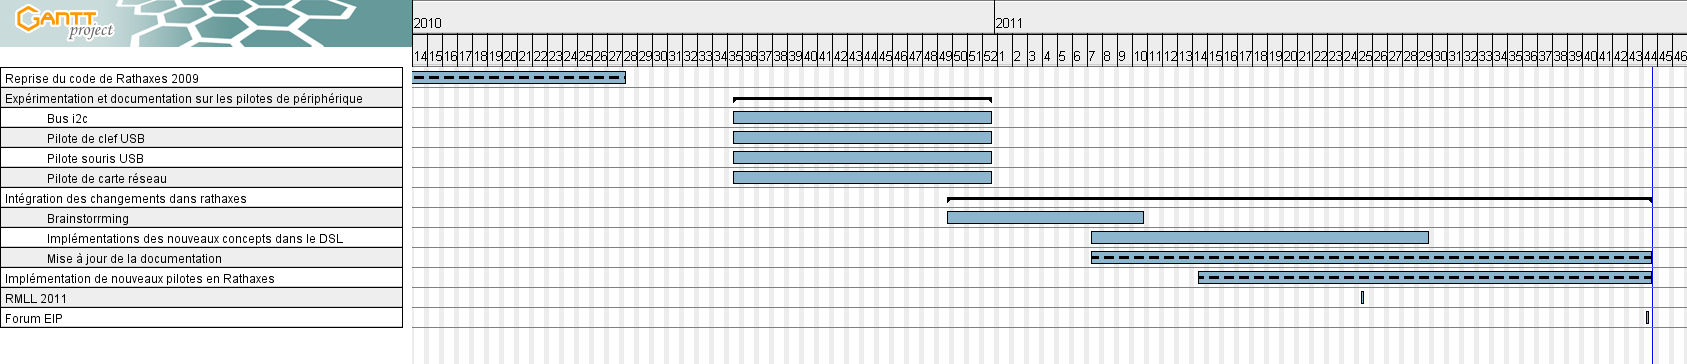
\includegraphics[angle=90,scale=0.35]{../images/gantt}

\end{center}

\begin{thebibliography}{9}

\bibitem{linux-tutorial}
The linux tutorial,
Device Driver Basic,\\
\url{http://www.linux-tutorial.info/modules.php?name=MContent&pageid=255}

\bibitem{GPLv3}
The Free Software Foundation,
\emph{GNU General Public License},\\
\url{http://www.gnu.org/licenses/gpl-3.0.html},\\
Version~3,
June~2007.

\bibitem{BSD}
University of California, Berkeley,
\emph{Simplified BSD License},\\
\url{http://www.opensource.org/licenses/bsd-license.php}.

\bibitem{CodeWorker}
A universal parsing tool \& a source code generator,\\
\url{http://codeworker.org/}.

\end{thebibliography}


\end{document}
